\chapter{Parametric Phased Array}
%\clearpage
\section{Introduction}
Parametric loudspeaker arrays are linear phased transducer arrays, which use the demodulation of ultrasound in air to generate a highly directional and steerable sound source. This effect was first discovered by Westerveld \cite{doi:10.1121/1.1918525} and used in a loudspeaker, the Audio Spotlight, by Masahide Yoneyama and Jun‐ichiroh Fujimoto \cite{doi:10.1121/1.389414}.

Why ultrasound generates a higher directivity is shown in Section \ref{3_sec:directivity}, how the demodulation works in \ref{3_sec:demodulation} and how signal processing tricks can be used to make everything steerable and of better quality is shown in \ref{3_Parametric_array_Sec:Modulation} and \ref{3_Parametric_array_Sec:Array_signal_processing}.
\section{Directivity of Ultrasound Transducers}\label{3_sec:directivity}
As already mentioned ultrasonic transducer produce a highly directional beam. In this chapter the mathematical foundations for this effect will be laid. 
The simplest model of a transducer is to think of it as a slit on which a incoming planar sound wave is diffracted on.\cite{alma99116706330905515} 
The far-field air pressure of a transducer in relation to the angle and the distance to the transducer can therefore be calculated as
\begin{equation}
    p(\varphi,r) 
    = 
    \frac{A}{r} \underbrace{\frac{\sin \left ( \frac{ks \sin \phi}{2}\right )}{ \frac{ks \sin \phi}{2}}}_{D_T(\varphi)}.
\end{equation}
Where the sinc function is better known as the directivity of the transducer. 
\begin{equation}
    D_T(\varphi) = \frac{\sin \left ( \frac{ks \sin \phi}{2}\right )}{ \frac{ks \sin \phi}{2}}
\end{equation}
This directivity for a $k = \frac{40 \, \text{kHz}}{343 \, \text{m/s}}$ and loudspeaker size of $a = 16 \, \text{mm}$ is shown in Figure \ref{2_subfig:single_slid_amp}. It is important to keep in mind that this directivity is just a model and the true directivity of a transducer can vary massively depending on the geometry of the transducers, especially as the angle increases.
\section{Demodulation Process}\label{3_sec:demodulation}
The most fundamental equation for modeling the non linear behaviour of air is the KZK (Khokhlov, Zabalotskaya and Kuznetsov) equation \cite{MIT_Ultrasound} given as
\begin{equation}
    \frac{\partial^2 p}{\partial z \partial \tau} 
    = 
    \frac{c_0}{2} \nabla^2_rp
    + 
    \frac{\delta}{2c_0^3}\frac{\partial^3 p}{\partial \tau^3} 
    + 
    \frac{\beta}{2\rho_0c_0^3}\frac{\partial^2 p^2}{\partial \tau^2}.
\end{equation}
Of which the analytical solutions can not be calculated.
However the solution can be approximated by first solving for the linear ultrasonic field $p_1$ by setting the nonlinear term to zero $\beta = 0$ and then solve for the nonlinear solution $p_2$ the final solution is then the superposition of these two fields $p = p_1 + p_2$.
The ultrasonic field $p_1$ is described by 
\begin{equation}
     \frac{\partial^2 p_1}{\partial z \partial \tau} 
    = 
    \frac{c_0}{2} \nabla^2_rp_1 
    + 
    \frac{\delta}{2c_0^3}\frac{\partial^3 p_1}{\partial \tau^3} 
\end{equation}
and this can now analytically be solved. 
This solution then can be used as an approximation for the non linear part of the equation
\begin{equation}
     \frac{\partial^2 p_2}{\partial z \partial \tau} 
    = 
    \frac{c_0}{2} \nabla^2_rp_2 
    + 
    \frac{\delta}{2c_0^3}\frac{\partial^3 p_2}{\partial \tau^3} 
    + 
    \frac{\beta}{2\rho_0c_0^3}\frac{\partial^2 p_1^2}{\partial \tau^2}
\end{equation}
which can now be solved near the axis analytically.
The resulting function $p_2$ turns out to be 
\begin{equation}
    p_2 = \frac{\beta P_0^2 a^2}{16 \rho_0 \alpha c_0^4 a^2}\frac{d^2}{dt^2} E^2(t)
\end{equation}
Where $E^2(t)$ is the enveloping of the output signal of the transducers. 
This means that the  pressure of the wave in the farfield is proportional to the second derivative of the squared modulated signal.
\begin{equation}
    p_2 \propto \frac{d^2}{dt^2} E^2(t)
\end{equation}
If the pressure now should be the desired audio signal f(t) the envelope of the output signal of the transducers has to be
\begin{equation}
    E(t) = \sqrt{\left ( 1 + m \int \int f(t)dt^2 \right )} =  \sqrt{\left ( 1 +x^2 \right )}.
\end{equation}
But it turns out that this is  impossible to accomplish because of the bandwidth of the ultrasonic transducers.
If $E(t)$ is written as a taylor approximation
\begin{equation}\label{3_eq:ideal_envelope}
    E(t) 
    = 
    \frac{1}{A} \left ( 1 + \frac{1}{2}x - \frac{1}{8}x^2 + \frac{1}{16}x^3 - \dots \right ) 
    =
    1 - \sum_{k=0}^\infty \frac{2}{k+1} \left ( \binom{2k}{k} \right) \left ( -\frac{x}{4}\right )^{k+1}.
\end{equation}
The spectrum $E_T(\omega)$ of the optimal signal is
\begin{equation}
    E_T(\omega) = \frac{1}{A} \left ( 1 + \frac{1}{2}X(w) - \frac{1}{8}\left (X(w) * X(w)\right ) \pm \dots \right ).
\end{equation}
This shows that $E_T(\omega)$ has an infinite bandwidth, because each correlation in frequency, or multiplication in time, doubles the bandwidth.
So an approximation for the envelope has to be found.
\section{Modulation}\label{3_Parametric_array_Sec:Modulation}
\begin{center}
    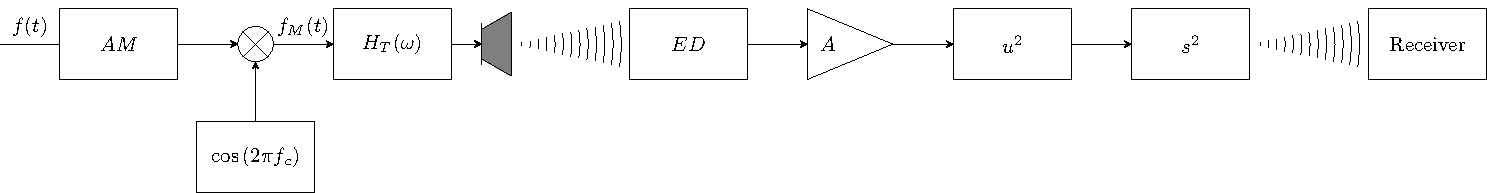
\includegraphics[width=\textwidth]{images/3_Parametric_array/Block_Diagram_Modulation.pdf}
\end{center}
As already mentioned if the ideal envelope, which can be seen in Equation \ref{3_eq:ideal_envelope}, should be emitted by the transducer they would have to have an infinite bandwidth because 
\begin{equation}
    U(\omega) = E_T(\omega) H_T(\omega).
\end{equation}
And because of this an approximation has to be made.
The two approximations that can be made for these envelope function discussed here are AM and MAM. 
\subsection{AM}
One possible approximation is to use normal amplitude modulation. The transmitted signal $g_{AM}(t)$ would be 
\begin{equation}
    g_{AM}(t) = h_T(t) * (1 + mf(t)).
\end{equation}
Often $H_T(\omega)$ is approximated to be $\frac{1}{s^2}$, which would cancel out the two derivatives
\begin{equation}
    f_{RX}(t) 
    = 
    Ag^2_{AM}(t) 
    =
    A(2mf + m^2f^2(t))
    =
   \underbrace{2Amf(t)}_{\text{Signal}} + \underbrace{2Am^2f^2(t)}_{\text{Distortion term}}.
\end{equation}
If the simplification of $H_T(\omega)$ is not made the spectrum of the received signal becomes
\begin{equation}
    F_{RX}(\omega) = 2A(mF(\omega)H(\omega) + m^2(F(\omega)*F(\omega))H(\omega))
\end{equation}
As one can see the modulation index $m$ is squared inside of the distortion term and only linear in the signal. This means that if the modulation index would be chosen small enough the distortion term would vanish, but the power of the signal would also be reduced significantly. 
\subsection{Modified Amplitude Modulation}
As seen if DSBAM is used there is a problematic distortion term. Modified Amplitude Modulation or MAM uses a similar idea to quadrature amplitude modulation to get rid of this problem \cite{MAM_Main_Paper} .
As the inphase component the input signal $1 + mf(t)$ with a DC offset is used and  as the quadrature component the signal $\sqrt{1 - m^2f^2(t)}$ is used. If now the output signal of the modulation $f_M(t)$ is calculated, as described in \ref{2_QAM_sec:QAM}, it turnes out to be
\begin{equation}
    f_M(t) = \sqrt{2 + 2mf(t)} \sin{\left(\omega_0 t + \arctan{ \left ( \frac{\sqrt{1 - m^2f^2(t)}}{1 + mf(t)} \right )} \right )}.
\end{equation}
If $H_T(\omega)$ is now again assumed to be $H_T(\omega) = \frac{1}{\omega^2}$ the signal turns out to be exactly what is should be. 

This would be a perfect modulation method but again because of the square root in the quadrature component this modulation can not be output by the transducers due to their limited bandwidth. However the basic idea still can be used. This is done by approximating the distortion terms with a taylor series
\begin{equation}
    Q(t) 
    = 
    \sqrt{1 - m^2f^2(t)}
    = 
    \sum_{i=0}^\infty \frac{(2i)!}{(1-2i) i!^2 4^i}m^{2i}g^{2i}(t) 
    \approx 
    \sum_{i=0}^m \frac{(2i)!}{(1-2i) i!^2 4^i}m^{2i}g^{2i}(t).
    \label{3_eq:mam_distortion_approx}
\end{equation}
Depending on the frequency response of the transducers the degree of the approximation $m$ can be chosen. The higher the degree of approximation gets the higher the bandwidth of the transducers have to be.
\newpage

\section{Array Signal Processing}\label{3_Parametric_array_Sec:Array_signal_processing}
The theory in this section is mostly taken from the book Fundamentals of Ultrasonic Phased Array \cite{alma99116706330905515}.
\subsection{Phased Array Beam Model}
To explain phenomena such as beamsteering and beamfocusing the phased array beam model has to be introduced.
 \begin{figure}[h!]
     \centering
     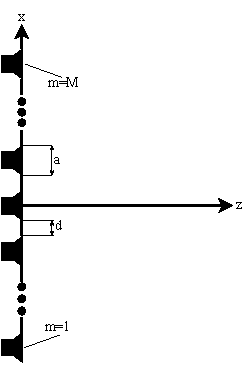
\includegraphics[width=0.4\textwidth]{images/3_Parametric_array/Loudspeaker_Arangement.pdf}
     \caption{Transducer arrangement}
     \label{3_Parametric_array_img:Transducer_Model}
 \end{figure}
Figure \ref{3_Parametric_array_img:Transducer_Model} shows the basic setup of a transducer array with M elements, where M is odd. Where the position of the mth element is given as \cite{alma99116706330905515} 
\begin{equation}\label{3.4_eq:simplified_xm}
    x_m 
    = 
    \left ( \frac{2m -1 - M}{2} \right ) \underbrace{(d + s)}_{c}
    =
    \left ( \frac{2m -1 - M}{2} \right ) c
\end{equation}
Where d is the distance between the transducers, a is the size of the transducers and c is known as the pinch of the array. 
The far field pressure of a single element can be calculated as \cite{alma99116706330905515}
\begin{equation}
    p_m(\textbf{x},\omega) 
    =
    \underbrace{\rho c V_0 \frac{k b}{N} \sqrt{\frac{2}{\pi i}}}_{C} D(\varphi_{m}) \frac{e^{j k b \Bar{r_m}}}{\sqrt{k b \Bar{r_m}}}  
\end{equation}
Where
\begin{equation}
    \Bar{r_m} 
    = 
    \sqrt{\left ( \frac{x}{b} - \frac{e_m}{b}\right )^2 + \left ( \frac{z}{b} \right )^2}
\end{equation}
and 
\begin{equation}
    \varphi_m = \sin^{-1}{\left ( \frac{x - e_m}{b \Bar{r_m}} \right )}
\end{equation}
If now each elements gets its own weighting factor $C_m$ and a phase delay $\Delta t_m$ the pressure at position $\Vec{x}$ of a wave with the frequency $\omega$ can be calulated as 
\begin{equation}
    p(\Vec{x},\omega) 
    = 
    \sum_{i=0}^M C_m e^{j\omega \Delta t_m} \underbrace{C D(\varphi_{m}) \frac{e^{j k b \Bar{r_m}}}{\sqrt{k b \Bar{r_m}}}}_{ p_m(\textbf{x},\omega)} 
\end{equation}
\subsubsection{Far Field}
If only the far field is of interest. Then $\Bar{r}_{m}$ can be simplified to \cite{alma99116706330905515}
\begin{equation}
    \Bar{r}_{m} = R - e_m \sin{\varphi}
\end{equation}
and $\varphi_m$ to
\begin{equation}
    \varphi_m = \varphi.
\end{equation}
So the pressure can be approximately written as
\begin{align}
    p(R,\varphi,\omega) 
    &= 
    C D(\varphi) \sum_{i=0}^M C_m e^{j\omega \Delta t_m} \underbrace{\frac{e^{j k R}}{\sqrt{k R}}}_{P(R)}e^{-jke_m\sin{(\varphi)}} \\
    &= 
    C D(\varphi) P(R) \sum_{i=0}^M C_m e^{j\omega \Delta t_m} e^{-jke_m\sin{(\varphi)}}
\end{align}
Or with \ref{3.4_eq:simplified_xm} as
\begin{equation}
    p(R,\varphi,\omega) 
    = 
    C D(\varphi) P(R) \underbrace{\sum_{i=0}^M C_m e^{j (\omega \Delta t_m -k \left ( \frac{2m -1 - M}{2} \right )s \sin{(\varphi)} )}}_{D_S(\bm{C}, \bm{\Delta t} , \varphi)}
    \label{3_eq:beam_model_final}
\end{equation}
This is the main model used to explain the directivity pattern of linear phased arrays and with using different weights $C_m$ and delays $t_m$ the behaviour can be explored. The sum can be understood as a directivity $D_s$ introduced by the delays and the weighting. 

As an example the weights $C_m = 1$ and $\Delta t_m = 0$ are set to which leads to
\begin{equation}
   D_s(\phi)
    = 
    e^{jks\left ( \frac{M+1}{2} \right )\sin{\phi} } \sum_{m=1}^M \left ( e^{-jks \sin{(\varphi)}} \right ) ^ m 
\end{equation}
This can be seen as a geometric series which can be written as 
\begin{align}
   \sum_{m=1}^M \left ( e^{-jks \sin{(\varphi)}} \right ) ^ m
    &= 
     e^{-jks \sin{(\varphi)}}\frac{1 - e^{-jks \sin{(\varphi) M }}}{1 - e^{-jks \sin{(\varphi)}}} \\
     &=
     e^{-jks\left ( \frac{M + 1}{2}\right ) \sin{(\varphi)}} \frac{\sin{\frac{Mks\sin{(\phi)}}{2}}}{\sin{\frac{ks\sin{(\varphi)}}{2}}}
\end{align}
So the array directivity  in relation to $R$,$\phi$ and $\omega$ can be described as
\begin{equation}
    D_s(\phi) 
    = 
    \frac{\sin{\frac{Mks\sin{(\phi)}}{2}}}{\sin{\frac{ks\sin{(\varphi)}}{2}}}
    \label{3_eq:directivity_no_delay}
\end{equation}
Since $k = \frac{2\pi}{\lambda}$, if $s = \lambda$ the directivity turnes out to be
\begin{equation}
    D_s(\phi) 
    = 
    \frac{\sin{\left ( M\pi\sin{(\phi)} \right )} }{ \sin{\left ( \pi\sin{(\varphi)}\right )}}
\end{equation}
in which the numerator and the denominator are only equal at zero and $2\pi$. So there is only one main lobe in the range between $-\pi/2$ and $\pi/2$. If this is not the case there are multiple lobes with the size of the main lobe.
\begin{figure}
    \begin{minipage}{0.49\textwidth}
    \centering
    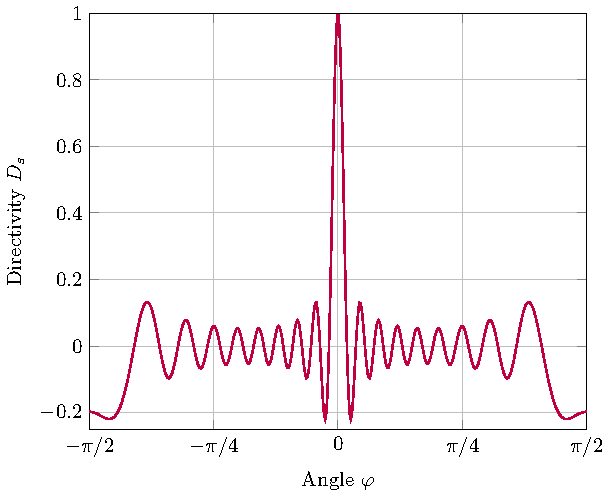
\includegraphics[width=\textwidth]{images/3_Parametric_array/Directivity_NoSteer_Lambda.pdf}
    \caption{Array directivity $s = \lambda$}
    \label{3_subfig:directivity_no_steer_lambda}
    \end{minipage}
    \begin{minipage}{0.49\textwidth}
    \centering
    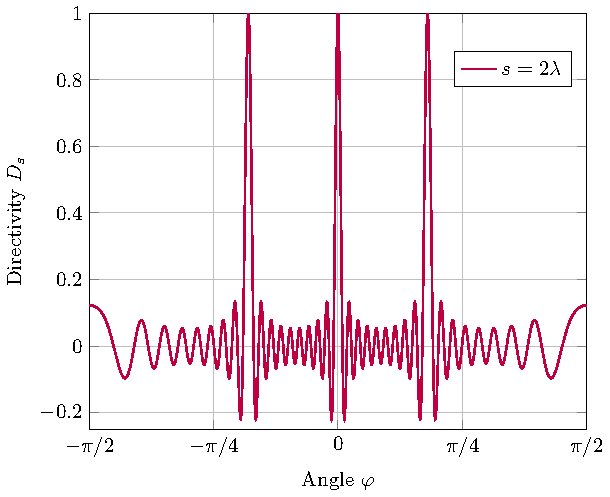
\includegraphics[width=\textwidth]{images/3_Parametric_array/Directivity_NoSteer_2Lambda.pdf}
    \caption{Array directivity $s = 2\lambda$}
     \label{3_subfig:directivity_no_steer_2lambda}
    \end{minipage}
\end{figure}

\subsection{Array Beamsteering}
The basic idea of beam steering is to delay the different channels in such a way that the wave fronts create a certain angle. This can be seen graphicaly in Figure \ref{3_fig:basic_idea_beamforming}.
\begin{figure}
    \centering
    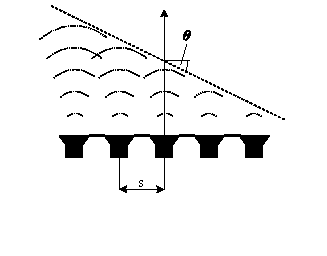
\includegraphics[trim=0mm 7mm 0mm 0mm, width=0.8\textwidth]{images/3_Parametric_array/Beamforming.pdf}
    \caption{Basic idea beamforming}
    \label{3_fig:basic_idea_beamforming}
\end{figure}
If the delays
\begin{equation}
    \Delta t_m = \frac{s \sin{\theta}}{c} \left ( \frac{2m - 1 - M}{2}\right ),
\end{equation}
where $\theta$ is the angle to steer and the weights $C_m = 1$ are inserted into Equation \ref{3_eq:beam_model_final}  
the array directivity $D_S$, after some algebra, is given as \cite{alma99116706330905515}
\begin{equation}
    D_S(1, \bm{\Delta t} , \varphi) 
    = 
    \frac{\sin{\frac{Mks(\sin{(\phi)} - \sin{(\theta)})}{2}}}{M\sin{\frac{ks(\sin{(\varphi)} - \sin{(\theta)})}{2}}}.
\end{equation}
This shows that the beamsteering just moves the the directivity calculated in \ref{3_eq:directivity_no_delay} around.  
This can be seen in Figure \ref{3_fig:directivity_beamsteering} for different steering angles.  
\begin{figure}
    \centering
    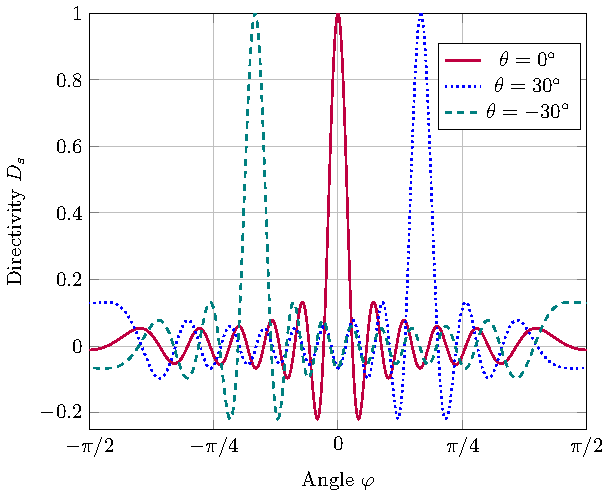
\includegraphics[width=0.7\textwidth]{images/3_Parametric_array/Directivity_Steer.pdf}
    \caption{Array directivity with different steering angles}
    \label{3_fig:directivity_beamsteering}
\end{figure}
\subsection{Beamfocusing}
To focus the beam at a certain radius $R_0$ the delays have to be chosen as
\begin{equation}
    \Delta t_m = \frac{s^2}{2R_0c}(m-1)(M-m).
\end{equation}
This generates delays which are shaped like a parabolic mirror which ensure that the waves exactly meet at the focus point, like shown in Figure \ref{3_fig:beamfocusing}.
\begin{figure}
    \centering
    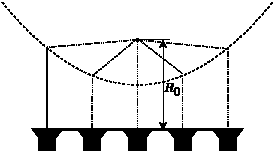
\includegraphics[width=0.7\textwidth]{images/3_Parametric_array/Beamfocusing.pdf}
    \caption{Basic idea beam focusing}
    \label{3_fig:beamfocusing}
\end{figure}
\subsection{Array Amplitude Weighting}
As explained in \ref{2_Acoustics_sec:diffraction_fourier} the diffraction process of a grid can be calculated via the fourier transform. If an array of transducers are used the function f(x) is a rectangular sequence. If this rectangular sequence is now sampled with a sampling width of $d$ then the signal is a rectangular window known from FIR filters. The main difference is now that the time axis was replaced by a spatial axis.
If now weights are applied to the different channels the rectangular window can be changed to other known windowing function, such as Hamming or Hann, and the same theories will hold for the main and side lobes. However the most used window in array signal processing is the dolph-chebyshev window.  
\subsubsection{Dolph-Chebyshev Window}
The Dolph-Chebyshev Window is a special window which minimizes the so called Chebyshev norm of the side lobes for a given main lobe width. The chebyshev norm is the maximum absolute value
\begin{equation}
    \min_{\omega, \sum \omega = 1} \left \{ \max \left[ | \text{Sidelobes}(W(\omega))\right | ]\right \}.
\end{equation}
The transform of the window can be written as
\begin{equation}
    W(\omega_k) = \frac{\cos{ \left [ M \cos^{-1}{\left ( \beta \cos{ \left (\frac{\pi k}{M} \right )} \right)}\right ]}}{\cosh{\left [ M \cosh^{-1}{\left ( \beta \right ) }\right ]}} \qquad k = 0,1,2, \dots, M-1
\end{equation}
Where M is the number of taps of the window and $\beta$ can be used to control the side lobe level.
The  \acrfull{idft} of $W(\omega_k)$ is now the Dolph-Chebyshev window $w(n)$.
The controlling of the side lobe level is often done by introducing another variable $\alpha$ which is connected to $\beta$ in the following way
\begin{equation}
    \beta = \cosh{\left [ \frac{1}{M} \cosh^{-1}{\left ( 10^{\alpha} \right ) } \right ]}.
\end{equation}
The maximum side lobe level is now given as
\begin{equation}
    \text{Side lobe level} = L_s =  -20\alpha [dB]
\end{equation}
Whereas the main lobe width is given as
\begin{equation}
    \omega_c = 2 \cos^{-1}{ \left ( \frac{1}{x_0} \right )} \qquad x_0 = \cosh{ \left [ \frac{\cosh^{-1}{\left ( 10^{\alpha} \right )}}{M-1}\right ]}.
\end{equation}
One can see that the higher the $\alpha$ is chosen the lower the maximum of the side lobes get, but the main lobe gets wider. \todo{Plot}





